\documentclass[12pt]{article}
\usepackage{fancyhdr}
\usepackage{amsmath,amsfonts,enumerate}
\usepackage{color,graphicx}
\usepackage{tikz}
\usepackage{pgfplots}
\usepackage{listings}
\usepackage{algorithm}
\usepackage{algorithmic}
\usetikzlibrary{arrows,positioning,shapes,calc,matrix}
\pagestyle{fancy}

% Define colors for answers
\definecolor{answercolor}{RGB}{0,100,0}
\definecolor{explanationcolor}{RGB}{0,0,139}

% Custom commands for answers
\newcommand{\answer}[1]{{\color{answercolor}\textbf{Answer:} #1}}
\newcommand{\explanation}[1]{{\color{explanationcolor}#1}}

%%%%%%%%%%%%%%%%%%%%%%%%%%%%%%%%%%%%%%%%%%%%%%%%%
% Course customization based on Professor's teaching
%%%%%%%%%%%%%%%%%%%%%%%%%%%%%%%%%%%%%%%%%%%%%%%%%
\newcommand{\masunitnumber}{CENG 403}
\newcommand{\examdate}{January 2025}
\newcommand{\academicyear}{2024-2025}
\newcommand{\semester}{I}
\newcommand{\coursename}{Deep Learning - CNN Visualization \& Classic Architectures - ANSWERED}
\newcommand{\numberofhours}{3}
%%%%%%%%%%%%%%%%%%%%%%%%%%%%%%%%%%%%%%%%%%%%%%%%%
% CUSTOM SPACING COMMANDS FOR ANSWER SPACES
%%%%%%%%%%%%%%%%%%%%%%%%%%%%%%%%%%%%%%%%%%%%%%%%%
\newcommand{\answerspace}[1]{\vspace{#1}}
\newcommand{\questionspace}{\vspace{3cm}}        
\newcommand{\subquestionspace}{\vspace{2.5cm}}   
\newcommand{\shortanswer}{\vspace{2cm}}          
\newcommand{\mediumanswer}{\vspace{3cm}}         
\newcommand{\longanswer}{\vspace{4cm}}           
\newcommand{\journalspace}{\vspace{4.5cm}}       
\newcommand{\codespace}{\vspace{5cm}}            
%%%%%%%%%%%%%%%%%%%%%%%%%%%%%%%%%%%%%%%%%%%%%%%%%
% Header setup
%%%%%%%%%%%%%%%%%%%%%%%%%%%%%%%%%%%%%%%%%%%%%%%%%
\lhead{}
\rhead{}
\chead{{\bf MIDDLE EAST TECHNICAL UNIVERSITY}}
\lfoot{}
\rfoot{}
\cfoot{}
\begin{document}
\setlength{\headsep}{5truemm}
\setlength{\headheight}{14.5truemm}
\setlength{\voffset}{-0.45truein}
\renewcommand{\headrulewidth}{0.0pt}
\begin{center}
SEMESTER \semester\ EXAMINATION \academicyear
\end{center}
\begin{center}
{\bf \masunitnumber\ -- \coursename}
\end{center}
\vspace{20truemm}
\noindent \examdate\hspace{45truemm} TIME ALLOWED: \numberofhours\ HOURS
\vspace{19truemm}
\hrule
\vspace{19truemm}
\noindent\underline{INSTRUCTIONS TO CANDIDATES}
\vspace{8truemm}
%%%%%%%%%%%%%%%%%%%%%%%%%%%%%%%%%%%%%%%%%%%%%%%%%%%%%%
% Instructions based on professor's emphasis
%%%%%%%%%%%%%%%%%%%%%%%%%%%%%%%%%%%%%%%%%%%%%%%%%%%%%%
\begin{enumerate}
\item This examination paper contains {\bf SIX (6)} questions and comprises 
{\bf EIGHT (8)} printed pages.
\item Answer all questions. 
The marks for each question are indicated at the beginning of each question.
\item Answer each question beginning on a {\bf FRESH} page of the answer book.
\item This {\bf IS NOT an OPEN BOOK} exam.
\item Show clear reasoning for your answers, especially intuitive explanations.
\item For architectural diagrams, draw clear components and explain design choices.
\item Connect concepts to examples discussed in lectures where relevant.
\item Explain the practical implications of design decisions.
\end{enumerate}
%%%%%%%%%%%%%%%%%%%%%%%%%%%%%%%%%%%%%%%%%%%%%%%%%
% New page for questions
%%%%%%%%%%%%%%%%%%%%%%%%%%%%%%%%%%%%%%%%%%%%%%%%%
\newpage
\lhead{}
\rhead{\masunitnumber}
\chead{}
\lfoot{}
\cfoot{\thepage}
\rfoot{}
\setlength{\footskip}{45pt}
%%%%%%%%%%%%%%%%%%%%%%%%%%%%%%%%%%%%%%%%%%%%%%%%%%
% EXAM QUESTIONS BASED ON PROFESSOR'S TEACHING
%%%%%%%%%%%%%%%%%%%%%%%%%%%%%%%%%%%%%%%%%%%%%%%%%%

\paragraph{Question 1. Class Activation Maps and Global Average Pooling}{\hfill (25 marks)}\\
Based on the professor's explanation: "Each channel actually specializes in capturing one part or maybe the whole part of an object... it functions as a confidence map over pixels."

\begin{enumerate}[(a)]
    \item The professor explained that global average pooling forces each channel to specialize. Explain how class activation maps exploit this property to visualize what the network is "paying attention to." Include the mathematical process of weighting channels. \hfill (10 marks)
    
    \answer{Class Activation Maps (CAM) exploit the channel specialization property of Global Average Pooling to create spatial visualizations showing which regions the network considers important for each class.}
    
    \explanation{
    \textbf{Channel Specialization with Global Average Pooling:}
    
    When using Global Average Pooling, each channel in the final convolutional layer learns to specialize as a "confidence map" for detecting specific semantic concepts. This happens because:
    
    The final classification layer uses weights $w_{k,c}$ to combine channel activations:
    $$y_c = \sum_{k=1}^K w_{k,c} \cdot \text{GAP}(f_k)$$
    
    where $\text{GAP}(f_k) = \frac{1}{H \times W} \sum_{i,j} f_k(i,j)$ is the global average of channel $k$.
    
    To maximize class $c$ score, the network learns to make channel $k$ have high activations wherever objects relevant to class $c$ appear, and low activations elsewhere.
    
    \textbf{Class Activation Map Generation:}
    
    For a given class $c$, the CAM is computed as:
    $$\text{CAM}_c(i,j) = \sum_{k=1}^K w_{k,c} \cdot f_k(i,j)$$
    
    This creates a spatial heatmap where:
    \begin{itemize}
        \item High values indicate regions important for class $c$
        \item Each pixel's importance is a weighted combination of all channel activations
        \item The weights $w_{k,c}$ are learned during training for classification
    \end{itemize}
    
    \textbf{Mathematical Process:}
    1. Forward pass through CNN to get final conv layer activations $f_k(i,j)$
    2. Use learned classification weights $w_{k,c}$ 
    3. Compute weighted sum across channels for each spatial location
    4. Upscale to input image resolution if needed
    5. Overlay on original image as heatmap
    
    The key insight is that GAP forces channels to become semantic detectors, and CAM visualizes how these detectors vote for each class across the image.
    }
    
    \item Compare class activation maps with Grad-CAM as described by the professor. Explain why Grad-CAM replaces learned weights with "summation of gradients with respect to the channel" and how this makes the visualization "input dependent." \hfill (10 marks)
    
    \answer{Grad-CAM generalizes CAM by replacing fixed learned weights with input-specific gradient information, enabling visualization for any CNN architecture without requiring Global Average Pooling.}
    
    \explanation{
    \textbf{Key Differences Between CAM and Grad-CAM:}
    
    \textbf{CAM Limitations:}
    \begin{itemize}
        \item Requires Global Average Pooling architecture
        \item Uses fixed learned weights $w_{k,c}$ from classification layer
        \item Cannot be applied to networks with fully connected layers
        \item Same importance weights used regardless of input image
    \end{itemize}
    
    \textbf{Grad-CAM Solution:}
    
    Instead of using learned weights $w_{k,c}$, Grad-CAM computes:
    $$\alpha_k^c = \frac{1}{Z} \sum_i \sum_j \frac{\partial y^c}{\partial A_{i,j}^k}$$
    
    where:
    \begin{itemize}
        \item $y^c$ is the score for class $c$
        \item $A_{i,j}^k$ is the activation at spatial location $(i,j)$ in channel $k$
        \item $\alpha_k^c$ represents the importance of channel $k$ for class $c$ for this specific input
    \end{itemize}
    
    The Grad-CAM heatmap is:
    $$L_{\text{Grad-CAM}}^c = \text{ReLU}\left(\sum_k \alpha_k^c A^k\right)$$
    
    \textbf{Why Gradients Make It Input-Dependent:}
    
    The gradients $\frac{\partial y^c}{\partial A_{i,j}^k}$ capture how much a small change in channel $k$'s activation would affect the class $c$ score for the current input. This means:
    
    \begin{itemize}
        \item Different inputs produce different gradient patterns
        \item The importance weights $\alpha_k^c$ adapt to what the network is actually using for this specific prediction
        \item More relevant channels get higher weights for inputs where they're discriminative
        \item Less relevant channels get lower weights when they don't contribute to the decision
    \end{itemize}
    
    \textbf{Practical Advantages:}
    \begin{enumerate}
        \item \textbf{Architecture Flexibility:} Works with any CNN, including those with FC layers
        \item \textbf{Input Specificity:} Highlights features actually used for each prediction
        \item \textbf{Layer Flexibility:} Can visualize any convolutional layer, not just the last one
        \item \textbf{Better Localization:} Often provides more precise localization than CAM
    \end{enumerate}
    
    The gradient information tells us "for this specific input, how important is each channel for the predicted class," making the visualization much more informative and reliable.
    }
    
    \item The professor mentioned that "if you do this with a CNN that has fully connected layers you are not going to get such activation maps." Explain why global average pooling is essential for class activation maps and why fully connected layers prevent this visualization. \hfill (5 marks)
    
    \answer{Fully connected layers destroy spatial information by flattening feature maps into vectors, making it impossible to trace back class-specific importance to spatial locations in the original image.}
    
    \explanation{
    \textbf{Why Global Average Pooling Enables CAM:}
    
    GAP preserves the connection between spatial locations and class predictions:
    
    \begin{itemize}
        \item Each channel $f_k(i,j)$ maintains spatial coordinates $(i,j)$
        \item The classification layer directly uses channel averages: $y_c = \sum_k w_{k,c} \cdot \text{GAP}(f_k)$
        \item We can "reverse" this process: $\text{CAM}_c(i,j) = \sum_k w_{k,c} \cdot f_k(i,j)$
        \item This shows exactly which spatial locations contribute to each class score
    \end{itemize}
    
    \textbf{Why Fully Connected Layers Break CAM:}
    
    FC layers perform: $h = W \cdot \text{flatten}(f) + b$
    
    This creates several problems:
    \begin{enumerate}
        \item \textbf{Spatial Information Loss:} Flattening converts $f_k(i,j)$ into a 1D vector, losing all spatial structure
        \item \textbf{Mixed Spatial Responses:} Each FC neuron receives input from ALL spatial locations across ALL channels
        \item \textbf{No Direct Mapping:} Cannot trace how specific spatial locations influence the final prediction
        \item \textbf{Complex Interactions:} Multiple FC layers create complex non-linear transformations that obscure spatial contributions
    \end{enumerate}
    
    \textbf{Mathematical Explanation:}
    
    With GAP: $y_c = \sum_k w_{k,c} \cdot \frac{1}{HW}\sum_{i,j} f_k(i,j)$ 
    
    This can be rewritten as: $y_c = \frac{1}{HW} \sum_{i,j} \sum_k w_{k,c} \cdot f_k(i,j) = \frac{1}{HW} \sum_{i,j} \text{CAM}_c(i,j)$
    
    With FC layers: $y_c = g(\text{FC layers}(\text{flatten}(f)))$
    
    There's no simple way to decompose this back to spatial locations because the FC transformation mixes information from all spatial positions in complex ways.
    
    This is why CAM requires GAP architecture, and why Grad-CAM was developed to handle networks with FC layers by using gradient information instead.
    }
\end{enumerate}

\newpage
\paragraph{Question 2. Feature Inversion and Network Understanding}{\hfill (22 marks)}\\
The professor discussed: "Given the feature vector for X we can try to generate an image whose feature vector is similar to that image."

\begin{enumerate}[(a)]
    \item Formulate the feature inversion optimization problem as the professor described. Explain why this is useful for understanding "what the CNN is doing" and "what level of detail it has kept and captured at different layers." \hfill (8 marks)
    
    \answer{Feature inversion reconstructs images from feature representations by optimizing pixel values to match target activations, revealing what information is preserved at different network layers.}
    
    \explanation{
    \textbf{Feature Inversion Optimization Problem:}
    
    Given a target feature vector $\phi_l(x_0)$ from layer $l$ of a CNN, find an image $x^*$ such that:
    
    $$x^* = \arg\min_x ||\phi_l(x) - \phi_l(x_0)||_2^2 + \lambda \mathcal{R}(x)$$
    
    where:
    \begin{itemize}
        \item $\phi_l(x)$ is the feature representation of image $x$ at layer $l$
        \item $\phi_l(x_0)$ is the target feature vector (from original image $x_0$)
        \item $\mathcal{R}(x)$ are regularization terms to ensure natural-looking images
        \item $\lambda$ controls the regularization strength
    \end{itemize}
    
    \textbf{Optimization Process:}
    1. Initialize $x$ randomly (usually Gaussian noise)
    2. Forward pass: compute $\phi_l(x)$
    3. Compute loss: $\mathcal{L} = ||\phi_l(x) - \phi_l(x_0)||_2^2$
    4. Backward pass: compute $\frac{\partial \mathcal{L}}{\partial x}$
    5. Update $x$ using gradient descent: $x \leftarrow x - \alpha \frac{\partial \mathcal{L}}{\partial x}$
    6. Repeat until convergence
    
    \textbf{Understanding "What the CNN is Doing":}
    
    Feature inversion reveals:
    \begin{enumerate}
        \item \textbf{Information Content:} What visual information is encoded in each layer's features
        \item \textbf{Invariances:} What transformations the network considers equivalent
        \item \textbf{Selectivity:} Which visual patterns activate specific neurons
        \item \textbf{Hierarchical Processing:} How representations change across layers
    \end{enumerate}
    
    \textbf{Layer-by-Layer Analysis:}
    
    By performing inversion at different layers, we understand:
    \begin{itemize}
        \item \textbf{Early Layers:} Preserve low-level details (edges, textures, colors)
        \item \textbf{Middle Layers:} Capture mid-level patterns (shapes, object parts)
        \item \textbf{Late Layers:} Focus on high-level semantic content, lose spatial details
    \end{itemize}
    
    This helps us understand the progressive abstraction process in CNNs.
    }
    
    \item The professor showed reconstructions from different CNN layers. Explain his observation: "In the earlier layers information is redundant and we are able to capture the low-level details... when you go up in the network low-level details are lost." \hfill (8 marks)
    
    \answer{Layer-wise reconstructions reveal a trade-off between low-level detail preservation and high-level semantic understanding as we progress through the network hierarchy.}
    
    \explanation{
    \textbf{Early Layer Reconstructions:}
    
    \textbf{High Detail Preservation:}
    \begin{itemize}
        \item Reconstructions are nearly pixel-perfect copies of originals
        \item Preserve fine textures, exact colors, and precise edge locations
        \item Can recover exact spatial arrangements and small-scale patterns
        \item Information content is high and redundant
    \end{itemize}
    
    \textbf{Why Information is "Redundant":}
    Early layers capture raw visual information with high fidelity:
    \begin{itemize}
        \item Adjacent pixels are highly correlated
        \item Local patterns repeat across the image
        \item Network hasn't yet performed significant dimensionality reduction
        \item Features still maintain direct correspondence to pixel values
    \end{itemize}
    
    \textbf{Later Layer Reconstructions:}
    
    \textbf{Loss of Low-Level Details:}
    \begin{itemize}
        \item Reconstructions lose fine textures and exact colors
        \item Spatial locations become approximate rather than precise
        \item Background details often become blurred or missing
        \item Overall shape and semantic content preserved
    \end{itemize}
    
    \textbf{Information Transformation Process:}
    
    As we progress through layers:
    
    1. \textbf{Pooling Operations:} Reduce spatial resolution, losing precise location information
    2. \textbf{Non-linear Activations:} Introduce information bottlenecks
    3. \textbf{Increasing Receptive Fields:} Aggregate information over larger regions
    4. \textbf{Semantic Specialization:} Neurons become selective for high-level concepts
    
    \textbf{Mathematical Perspective:}
    
    Information content decreases with depth:
    $$I(\text{Image}; \phi_1) > I(\text{Image}; \phi_2) > ... > I(\text{Image}; \phi_L)$$
    
    But task-relevant information is preserved:
    $$I(\text{Class}; \phi_1) < I(\text{Class}; \phi_2) < ... < I(\text{Class}; \phi_L)$$
    
    \textbf{Practical Implications:}
    \begin{itemize}
        \item \textbf{Transfer Learning:} Early layers transfer well because they capture universal visual features
        \item \textbf{Feature Extraction:} Late layers better for semantic tasks, early layers for texture/style tasks
        \item \textbf{Network Design:} Need to balance detail preservation with semantic understanding
    \end{itemize}
    }
    
    \item The professor mentioned regularization terms to make generated images "visually pleasing." List and explain the regularization terms he discussed for controlling "smoothness" and ensuring "neighboring pixels have similar intensities." \hfill (6 marks)
    
    \answer{Regularization terms in feature inversion enforce natural image statistics to produce visually coherent reconstructions instead of noisy artifacts.}
    
    \explanation{
    \textbf{Total Variation (TV) Regularization:}
    
    Promotes spatial smoothness by penalizing large intensity differences between neighboring pixels:
    
    $$\mathcal{R}_{TV}(x) = \sum_{i,j} \left[ (x_{i+1,j} - x_{i,j})^2 + (x_{i,j+1} - x_{i,j})^2 \right]^{\beta/2}$$
    
    where $\beta = 1$ (L1) or $\beta = 2$ (L2).
    
    \textbf{Effect:} Encourages neighboring pixels to have similar intensities, reducing noise and creating smoother transitions.
    
    \textbf{L2 Pixel Norm Regularization:}
    
    Controls overall image magnitude:
    $$\mathcal{R}_{L2}(x) = ||x||_2^2 = \sum_{i,j} x_{i,j}^2$$
    
    \textbf{Effect:} Prevents pixel values from becoming arbitrarily large, keeping them in reasonable ranges.
    
    \textbf{Natural Image Prior:}
    
    Encourages reconstructions to follow natural image statistics:
    $$\mathcal{R}_{\text{prior}}(x) = -\log P(x)$$
    
    where $P(x)$ is a learned prior over natural images.
    
    \textbf{Alpha Norm Regularization:}
    
    Promotes sparsity in pixel values:
    $$\mathcal{R}_{\alpha}(x) = \sum_{i,j} |x_{i,j}|^\alpha$$
    
    where $\alpha < 2$ (commonly $\alpha = 6$).
    
    \textbf{Combined Objective:}
    
    The full optimization becomes:
    $$\min_x ||\phi_l(x) - \phi_l(x_0)||_2^2 + \lambda_1 \mathcal{R}_{TV}(x) + \lambda_2 \mathcal{R}_{L2}(x) + \lambda_3 \mathcal{R}_{\alpha}(x)$$
    
    \textbf{Practical Effects:}
    \begin{itemize}
        \item \textbf{Without regularization:} High-frequency noise, unnatural artifacts
        \item \textbf{With regularization:} Smooth, natural-looking images that preserve semantic content
        \item \textbf{Balance is crucial:} Too much regularization loses important details, too little creates artifacts
    \end{itemize}
    
    These regularization terms are essential because the feature matching objective alone can be satisfied by many unnatural images with high-frequency noise.
    }
\end{enumerate}

\newpage
\paragraph{Question 3. Adversarial Attacks}{\hfill (23 marks)}\\
Based on the professor's explanation: "We can generate a noise image that's called R with a very small magnitude such that when you add this noise image to the original image human eye is not able to visually distinguish this from the original."

\begin{enumerate}[(a)]
    \item Formulate the adversarial attack optimization problem as described by the professor. Distinguish between "targeted attack" (where "we have a target class in mind") and "untargeted attack" (where "as long as the correct class is not predicted it doesn't matter"). \hfill (8 marks)
    
    \answer{Adversarial attacks find minimal perturbations that fool neural networks while remaining imperceptible to humans, with different objectives for targeted versus untargeted scenarios.}
    
    \explanation{
    \textbf{General Adversarial Attack Formulation:}
    
    Given an original image $x$ with true class $y$, find a perturbation $r$ such that:
    
    $$x' = x + r$$
    
    where:
    \begin{itemize}
        \item $f(x') \neq y$ (misclassification occurs)
        \item $||r||_p \leq \epsilon$ (perturbation is small)
        \item $x'$ is visually indistinguishable from $x$ to humans
    \end{itemize}
    
    \textbf{Untargeted Attack:}
    
    Goal: Make the network predict any class except the correct one.
    
    $$\min_{r} ||r||_p \text{ subject to } f(x + r) \neq y \text{ and } x + r \in [0,1]^n$$
    
    Alternative formulation (maximizing loss):
    $$\max_{r} \mathcal{L}(f(x + r), y) \text{ subject to } ||r||_p \leq \epsilon$$
    
    where $\mathcal{L}$ is the classification loss (e.g., cross-entropy).
    
    \textbf{Targeted Attack:}
    
    Goal: Make the network predict a specific target class $t \neq y$.
    
    $$\min_{r} ||r||_p \text{ subject to } f(x + r) = t \text{ and } x + r \in [0,1]^n$$
    
    Alternative formulation (minimizing target loss):
    $$\min_{r} \mathcal{L}(f(x + r), t) \text{ subject to } ||r||_p \leq \epsilon$$
    
    \textbf{Key Differences:}
    
    \begin{itemize}
        \item \textbf{Untargeted:} Easier to achieve, any misclassification is success
        \item \textbf{Targeted:} Harder to achieve, must fool network toward specific class
        \item \textbf{Untargeted:} Often requires smaller perturbations
        \item \textbf{Targeted:} May require larger perturbations to reach specific target
    \end{itemize}
    
    \textbf{Common Attack Methods:}
    
    \textbf{Fast Gradient Sign Method (FGSM):}
    $$r = \epsilon \cdot \text{sign}(\nabla_x \mathcal{L}(f(x), y))$$
    
    \textbf{Projected Gradient Descent (PGD):}
    Iterative refinement with projection to constraint set.
    
    The key insight is that small, carefully crafted perturbations can exploit the high-dimensional nature of neural network decision boundaries.
    }
    
    \item Explain the difference between "white box approach" and "black box approach" for generating adversarial attacks. Describe the professor's explanation of using a "proxy network that mimics the predictions of the blackbox model." \hfill (8 marks)
    
    \answer{White box attacks have full access to model internals while black box attacks only observe outputs, requiring different strategies like proxy networks for gradient estimation.}
    
    \explanation{
    \textbf{White Box Approach:}
    
    \textbf{Available Information:}
    \begin{itemize}
        \item Complete model architecture
        \item All learned parameters (weights and biases)
        \item Activation functions and layer types
        \item Access to gradients via backpropagation
    \end{itemize}
    
    \textbf{Attack Strategy:}
    \begin{itemize}
        \item Directly compute gradients: $\nabla_x \mathcal{L}(f(x), y)$
        \item Use gradient-based optimization methods (FGSM, PGD, C&W)
        \item Can craft highly effective attacks with minimal perturbations
        \item Fast and computationally efficient
    \end{itemize}
    
    \textbf{Mathematical Process:}
    $$r^{(t+1)} = \Pi_{\epsilon}\left(r^{(t)} + \alpha \cdot \text{sign}(\nabla_x \mathcal{L}(f(x + r^{(t)}), y))\right)$$
    
    where $\Pi_{\epsilon}$ projects to the constraint set.
    
    \textbf{Black Box Approach:}
    
    \textbf{Limited Information:}
    \begin{itemize}
        \item Only access to model outputs (predictions/probabilities)
        \item No knowledge of architecture or parameters
        \item Cannot compute gradients directly
        \item Must treat model as a "black box" function
    \end{itemize}
    
    \textbf{Attack Strategies:}
    
    \textbf{1. Query-Based Methods:}
    \begin{itemize}
        \item Estimate gradients using finite differences
        \item $\frac{\partial f}{\partial x_i} \approx \frac{f(x + \delta e_i) - f(x - \delta e_i)}{2\delta}$
        \item Requires many queries to the target model
        \item Computationally expensive and detectable
    \end{itemize}
    
    \textbf{2. Proxy Network Approach (Professor's Explanation):}
    
    \textbf{Strategy:}
    1. Train a proxy network $g(x)$ to mimic the black box model $f(x)$
    2. Use the proxy for white box attacks: compute $\nabla_x \mathcal{L}(g(x), y)$
    3. Apply the adversarial examples to the original black box model
    4. Rely on \textbf{transferability} of adversarial examples
    
    \textbf{Proxy Training Process:}
    \begin{itemize}
        \item Collect input-output pairs from the black box: $\{(x_i, f(x_i))\}$
        \item Train proxy network: $\min_\theta \sum_i \mathcal{L}(g(x_i; \theta), f(x_i))$
        \item Use proxy for gradient computation
    \end{itemize}
    
    \textbf{Transferability Principle:}
    Adversarial examples often transfer between different models due to:
    \begin{itemize}
        \item Shared decision boundary properties
        \item Similar learned representations
        \item Common vulnerabilities in neural architectures
    \end{itemize}
    
    \textbf{Advantages and Limitations:}
    
    \textbf{White Box:}
    \begin{itemize}
        \item \textbf{Pros:} Highly effective, computationally efficient
        \item \textbf{Cons:} Requires full model access (unrealistic in practice)
    \end{itemize}
    
    \textbf{Black Box:}
    \begin{itemize}
        \item \textbf{Pros:} Realistic attack scenario, works on deployed models
        \item \textbf{Cons:} Lower success rates, requires more computation or queries
    \end{itemize}
    
    The proxy approach is particularly clever because it transforms a black box problem into a white box problem using transferability.
    }
    
    \item The professor discussed serious implications: autonomous cars could "misdetect a traffic sign" or "miss a crossing." Explain why adversarial robustness is challenging, including the professor's point about decision boundaries and the "trade-off between robustness and accuracy." \hfill (7 marks)
    
    \answer{Adversarial robustness is fundamentally challenging due to the high-dimensional nature of neural network decision boundaries and the inherent trade-off between fitting training data accurately and being robust to perturbations.}
    
    \explanation{
    \textbf{High-Dimensional Decision Boundary Problem:}
    
    In high-dimensional input spaces (e.g., images with thousands of pixels):
    \begin{itemize}
        \item Decision boundaries have enormous surface area
        \item Most points are close to some decision boundary
        \item Small perturbations can easily cross boundaries
        \item Networks learn complex, non-linear decision surfaces
    \end{itemize}
    
    \textbf{Mathematical Insight:}
    For an $n$-dimensional input space, the volume near decision boundaries grows exponentially with $n$. This means most natural inputs are vulnerable to small adversarial perturbations.
    
    \textbf{Fundamental Trade-off: Robustness vs. Accuracy:}
    
    \textbf{Accuracy Objective:}
    $$\min_\theta \mathbb{E}_{(x,y) \sim \mathcal{D}}[\mathcal{L}(f(x; \theta), y)]$$
    
    This encourages the model to fit the training distribution precisely.
    
    \textbf{Robustness Objective:}
    $$\min_\theta \mathbb{E}_{(x,y) \sim \mathcal{D}}\left[\max_{||r|| \leq \epsilon} \mathcal{L}(f(x + r; \theta), y)\right]$$
    
    This requires the model to be correct even under worst-case perturbations.
    
    \textbf{Why They Conflict:}
    
    \begin{enumerate}
        \item \textbf{Overfitting to Training Data:} High accuracy models may rely on spurious correlations
        \item \textbf{Sharp Decision Boundaries:} Accurate models often have sharp boundaries that are easy to cross
        \item \textbf{Feature Brittleness:} Models may rely on features that are not robust to small changes
        \item \textbf{Capacity Limitations:} Finite model capacity must choose between fitting data and being robust
    \end{enumerate}
    
    \textbf{Safety-Critical Applications:}
    
    \textbf{Autonomous Vehicles:}
    \begin{itemize}
        \item \textbf{Stop Sign Attack:} Stickers on stop signs could cause misclassification as speed limit signs
        \item \textbf{Pedestrian Detection:} Adversarial patches could make pedestrians "invisible" to detection systems
        \item \textbf{Lane Detection:} Road markings could be adversarially modified
    \end{itemize}
    
    \textbf{Medical Diagnosis:}
    \begin{itemize}
        \item Small changes to medical images could flip diagnosis
        \item Could lead to missed diseases or false positives
        \item Life-or-death consequences from misclassification
    \end{itemize}
    
    \textbf{Why Robustness is Fundamentally Hard:}
    
    \textbf{1. Curse of Dimensionality:}
    In high dimensions, "small" perturbations can be large in some directions.
    
    \textbf{2. Distribution Mismatch:}
    Adversarial examples are outside the training distribution but within the input space.
    
    \textbf{3. Gradient-Based Learning:}
    Standard training optimizes for average performance, not worst-case robustness.
    
    \textbf{4. Computational Constraints:}
    Robust training requires solving expensive min-max optimization problems.
    
    \textbf{Current Approaches and Limitations:}
    \begin{itemize}
        \item \textbf{Adversarial Training:} Include adversarial examples in training, but expensive and may overfit
        \item \textbf{Certified Defense:} Provide mathematical guarantees, but only for small perturbations
        \item \textbf{Detection Methods:} Try to detect adversarial examples, but can be circumvented
    \end{itemize}
    
    The fundamental challenge is that we want models that are simultaneously:
    \begin{itemize}
        \item Accurate on natural data
        \item Robust to all possible small perturbations
        \item Computationally efficient
        \item Generalizable to new domains
    \end{itemize}
    
    These objectives are often in tension, making adversarial robustness one of the most challenging problems in deep learning.
    }
\end{enumerate}

\newpage
\paragraph{Question 4. AlexNet Architecture and Design}{\hfill (25 marks)}\\
The professor described AlexNet as "the 2012 ImageNet winner" with "60 million parameters" that had to be "split into two branches" because "they were not able to fit the whole network into a single GPU."

\begin{enumerate}[(a)]
    \item Analyze the AlexNet architecture as described by the professor. Explain why they used "a stride of four" in the first layer and why this "huge reduction in dimensionality" worked in early layers but "would lose performance if tried in the top of the network." \hfill (10 marks)
    
    \answer{AlexNet's aggressive stride-4 in the first layer exploits the high redundancy in raw pixel data to reduce computational load, but such aggressive reduction would be harmful in later layers where information becomes more semantic and less redundant.}
    
    \explanation{
    \textbf{AlexNet Architecture Overview:}
    
    \textbf{Layer Structure:}
    \begin{enumerate}
        \item Conv1: $11 \times 11$ kernels, stride=4, 96 filters
        \item MaxPool1: $3 \times 3$, stride=2  
        \item Conv2: $5 \times 5$ kernels, stride=1, 256 filters
        \item MaxPool2: $3 \times 3$, stride=2
        \item Conv3: $3 \times 3$ kernels, stride=1, 384 filters
        \item Conv4: $3 \times 3$ kernels, stride=1, 384 filters
        \item Conv5: $3 \times 3$ kernels, stride=1, 256 filters
        \item MaxPool3: $3 \times 3$, stride=2
        \item FC1: 4096 units
        \item FC2: 4096 units  
        \item FC3: 1000 units (ImageNet classes)
    \end{enumerate}
    
    \textbf{Why Stride=4 in First Layer Works:}
    
    \textbf{1. High Pixel Redundancy:}
    Natural images have high spatial correlation:
    \begin{itemize}
        \item Adjacent pixels are highly correlated (correlation coefficient $\sim 0.95$)
        \item Information is distributed redundantly across neighboring pixels
        \item Aggressive subsampling removes redundancy without losing essential information
    \end{itemize}
    
    \textbf{2. Computational Efficiency:}
    Input: $224 \times 224 \times 3 = 150,528$ values
    After stride-4 conv: $55 \times 55 \times 96 = 290,400$ values
    
    \textbf{Computation reduction:}
    \begin{itemize}
        \item Stride-1 would produce $214 \times 214 \times 96 = 4.4M$ values
        \item Stride-4 produces $55 \times 55 \times 96 = 0.29M$ values
        \item $15\times$ reduction in feature map size
        \item Massive reduction in subsequent computational cost
    \end{itemize}
    
    \textbf{3. Effective Receptive Field:}
    Large $11 \times 11$ kernels with stride-4 still capture sufficient local context while dramatically reducing spatial dimensions.
    
    \textbf{Why This Fails in Later Layers:}
    
    \textbf{1. Information Becomes Semantic:}
    \begin{itemize}
        \item Later layers encode high-level semantic features
        \item Each spatial location represents important object parts or relationships
        \item Aggressive pooling would destroy crucial semantic information
    \end{itemize}
    
    \textbf{2. Reduced Redundancy:}
    \begin{itemize}
        \item After several layers, redundancy is much lower
        \item Each feature map location contains unique, non-redundant information
        \item Pooling becomes information destructive rather than efficiency improving
    \end{itemize}
    
    \textbf{3. Spatial Relationships Matter:}
    \begin{itemize}
        \item Object part relationships become crucial for recognition
        \item Relative spatial positions encode important semantic information
        \item Aggressive reduction destroys these relationships
    \end{itemize}
    
    \textbf{Mathematical Perspective:}
    
    \textbf{Early layers:} $H(X) \approx H(\text{Subsample}(X))$ (entropy preserved)
    \textbf{Late layers:} $H(X) \gg H(\text{Subsample}(X))$ (significant information loss)
    
    This design principle - aggressive reduction early, conservative reduction late - became a fundamental CNN design pattern.
    }
    
    \item The professor found it "striking" that AlexNet filters showed specialization: one GPU learned "more or less color insensitive" filters while the other learned "more color selective filters." Explain this phenomenon and what it suggests about "group convolution." \hfill (8 marks)
    
    \answer{AlexNet's dual-GPU architecture accidentally discovered that splitting features into groups leads to specialized filter learning, laying the groundwork for modern group convolution techniques.}
    
    \explanation{
    \textbf{AlexNet's Dual-GPU Architecture:}
    
    Due to memory limitations (GPUs had only 3GB in 2012):
    \begin{itemize}
        \item Network split across two GPUs
        \item Each GPU handled half the filters (48 filters each in first layer)
        \item Limited communication between GPUs (only at certain layers)
        \item Forced independent learning in each branch
    \end{itemize}
    
    \textbf{Observed Filter Specialization:}
    
    \textbf{GPU 1 Filters:}
    \begin{itemize}
        \item Learned mostly grayscale, color-insensitive filters
        \item Focused on edges, textures, and luminance patterns
        \item Similar to traditional computer vision filters (Gabor, edge detectors)
        \item More "generic" visual feature detection
    \end{itemize}
    
    \textbf{GPU 2 Filters:}
    \begin{itemize}
        \item Learned highly color-selective filters
        \item Specialized in color patterns and chromatic information
        \item Complementary to GPU 1's achromatic processing
        \item More specialized for color-based discrimination
    \end{itemize}
    
    \textbf{Why This Specialization Occurred:}
    
    \textbf{1. Limited Communication:}
    \begin{itemize}
        \item Each GPU had to learn independently initially
        \item Forced diversification to avoid redundancy
        \item Each branch adapted to fill different functional roles
    \end{itemize}
    
    \textbf{2. Complementary Learning:}
    \begin{itemize}
        \item Network needed both luminance and chromatic information
        \item Division of labor emerged naturally
        \item Each GPU specialized where it could contribute most effectively
    \end{itemize}
    
    \textbf{3. Gradient Flow Optimization:}
    \begin{itemize}
        \item Each GPU received different gradient signals
        \item Specialized filters emerged to minimize overall network loss
        \item Natural feature differentiation occurred
    \end{itemize}
    
    \textbf{Connection to Group Convolution:}
    
    \textbf{Modern Group Convolution:}
    $$y_j = \sum_{i \in G_j} x_i * w_{i,j}$$
    
    where $G_j$ is the group of input channels connected to output channel $j$.
    
    \textbf{Benefits Suggested by AlexNet:}
    
    \textbf{1. Feature Diversification:}
    \begin{itemize}
        \item Groups force filters to learn different types of features
        \item Reduces redundancy in learned representations
        \item Increases overall network expressiveness
    \end{itemize}
    
    \textbf{2. Computational Efficiency:}
    \begin{itemize}
        \item Reduces parameters: full conv needs $C_{in} \times C_{out}$ connections
        \item Group conv needs $\frac{C_{in} \times C_{out}}{G}$ connections per group
        \item Maintains representational capacity with fewer parameters
    \end{itemize}
    
    \textbf{3. Improved Generalization:}
    \begin{itemize}
        \item Specialization prevents overfitting to specific features
        \item Forces network to learn more diverse, robust representations
        \item Similar to ensemble effects
    \end{itemize}
    
    \textbf{Modern Applications:}
    
    \textbf{ResNeXt:} Uses group convolution as a design principle
    \textbf{MobileNet:} Extreme case (depthwise convolution) where groups = channels
    \textbf{ShuffleNet:} Combines group convolution with channel shuffling
    
    \textbf{Key Insight:}
    AlexNet's accidental discovery showed that constraining connectivity can lead to more efficient and effective learning, inspiring an entire family of group-based architectures.
    }
    
    \item List the key techniques AlexNet used to "mitigate overfitting" as mentioned by the professor, including their approach to "manually" decaying learning rate when "the loss was not improving." \hfill (7 marks)
    
    \answer{AlexNet employed multiple overfitting mitigation strategies including data augmentation, dropout, weight decay, and manual learning rate scheduling based on loss plateau detection.}
    
    \explanation{
    \textbf{1. Data Augmentation:}
    
    \textbf{Image Translations and Horizontal Flips:}
    \begin{itemize}
        \item Random crops from $256 \times 256$ images to $224 \times 224$
        \item Horizontal reflections (50\% probability)
        \item Created multiple versions of each training image
        \item Effective dataset size increase: $\sim 2048\times$ (multiple crops × flip)
    \end{itemize}
    
    \textbf{PCA-based Color Augmentation:}
    \begin{itemize}
        \item Principal Component Analysis on RGB pixel values
        \item Add multiples of found principal components to images
        \item Changes color intensity and hue while preserving object identity
        \item Helped network become invariant to lighting changes
    \end{itemize}
    
    \textbf{2. Dropout Regularization:}
    
    \textbf{Application:}
    \begin{itemize}
        \item Applied to first two fully connected layers
        \item Dropout probability: 0.5
        \item Randomly set 50\% of neurons to zero during training
        \item All neurons active during testing (with appropriate scaling)
    \end{itemize}
    
    \textbf{Effect:}
    \begin{itemize}
        \item Prevents co-adaptation of neurons
        \item Forces network to learn more robust representations
        \item Reduces overfitting to specific neuron combinations
        \item Acts like training an ensemble of networks
    \end{itemize}
    
    \textbf{3. L2 Weight Decay:}
    
    \textbf{Implementation:}
    $$\mathcal{L}_{\text{total}} = \mathcal{L}_{\text{classification}} + \lambda \sum_i w_i^2$$
    
    \textbf{Parameters:}
    \begin{itemize}
        \item Weight decay coefficient: $\lambda = 0.0005$
        \item Applied to all trainable parameters
        \item Penalizes large weights to prevent overfitting
    \end{itemize}
    
    \textbf{4. Manual Learning Rate Scheduling:}
    
    \textbf{Strategy:}
    \begin{itemize}
        \item Initial learning rate: 0.01
        \item Monitor validation loss continuously
        \item When validation loss plateaus (stops improving), divide learning rate by 10
        \item Manual intervention by researchers watching training progress
        \item Process repeated until convergence
    \end{itemize}
    
    \textbf{Rationale:}
    \begin{itemize}
        \item High learning rate initially for fast convergence
        \item Lower learning rate when approaching minimum
        \item Prevents oscillation around optimal solution
        \item Allows fine-tuning of learned features
    \end{itemize}
    
    \textbf{5. Early Stopping (Implicit):}
    
    \textbf{Monitoring:}
    \begin{itemize}
        \item Tracked both training and validation accuracy
        \item Stopped training when validation performance degraded
        \item Prevented excessive overfitting to training set
    \end{itemize}
    
    \textbf{6. Architecture Choices for Regularization:}
    
    \textbf{Local Response Normalization:}
    \begin{itemize}
        \item Normalized responses across feature maps
        \item Implemented lateral inhibition mechanism
        \item Helped with generalization (though later found less effective)
    \end{itemize}
    
    \textbf{Overlapping Pooling:}
    \begin{itemize}
        \item Pool size 3×3 with stride 2 (overlapping)
        \item Slight regularization effect compared to non-overlapping
        \item Reduced top-1 error by 0.4\% and top-5 error by 0.3\%
    \end{itemize}
    
    \textbf{Historical Context:}
    
    These techniques were pioneering in 2012:
    \begin{itemize}
        \item Dropout was a relatively new technique
        \item Data augmentation not yet standard practice
        \item Manual learning rate scheduling was common (automatic schedulers came later)
        \item Combination of techniques was novel and effective
    \end{itemize}
    
    The success of these regularization techniques in AlexNet established many best practices that are still used in modern deep learning.
    }
\end{enumerate}

\newpage
\paragraph{Question 5. GoogleNet and Inception Modules}{\hfill (30 marks)}\\
The professor explained GoogleNet's contributions: reducing parameters "from 60 million in AlexNet to 4 million" while achieving better performance.

\begin{enumerate}[(a)]
    \item Explain the motivation for inception modules as described by the professor: "information can exist at multiple scales" and "if you use a fixed receptive field size at a layer actually you are restricting the type of information you can extract to only a fixed scale." \hfill (8 marks)
    
    \answer{Inception modules address the fundamental limitation that fixed kernel sizes can only capture information at a single scale, while real-world objects and features exist at multiple scales simultaneously.}
    
    \explanation{
    \textbf{Multi-Scale Information Problem:}
    
    \textbf{Real-World Visual Complexity:}
    \begin{itemize}
        \item Objects appear at different sizes in images
        \item Same object type can have varying scales (near vs. far cars)
        \item Important features exist at multiple granularities
        \item Fine details and coarse structures both matter for recognition
    \end{itemize}
    
    \textbf{Traditional CNN Limitation:}
    
    Each layer uses fixed kernel size (e.g., $3 \times 3$):
    \begin{itemize}
        \item Can only capture information at one spatial scale
        \item Receptive field grows layer by layer, but each layer is still scale-limited
        \item Forces network to choose between fine details and coarse patterns
        \item Suboptimal for objects that have both fine and coarse important features
    \end{itemize}
    
    \textbf{Scale Examples in Vision:}
    
    \textbf{Fine Scale ($1 \times 1, 3 \times 3$):}
    \begin{itemize}
        \item Texture patterns, edge details
        \item Local color variations
        \item Small discriminative features
    \end{itemize}
    
    \textbf{Medium Scale ($5 \times 5$):}
    \begin{itemize}
        \item Object parts (eyes, wheels, etc.)
        \item Medium-sized patterns
        \item Spatial relationships between local features
    \end{itemize}
    
    \textbf{Coarse Scale (Pooling):}
    \begin{itemize}
        \item Global shape information
        \item Spatial layout of major components
        \item Context and background relationships
    \end{itemize}
    
    \textbf{Inception Solution - Multi-Scale Processing:}
    
    \textbf{Parallel Processing:}
    Instead of choosing one kernel size, use multiple kernel sizes in parallel:
    \begin{itemize}
        \item $1 \times 1$ convolutions for point-wise features
        \item $3 \times 3$ convolutions for local patterns
        \item $5 \times 5$ convolutions for larger patterns
        \item $3 \times 3$ max pooling for spatial reduction
    \end{itemize}
    
    \textbf{Information Fusion:}
    \begin{itemize}
        \item All scales processed simultaneously from same input
        \item Results concatenated to preserve all scale information
        \item Network learns to combine multi-scale features optimally
        \item No information loss from scale selection
    \end{itemize}
    
    \textbf{Benefits:}
    
    \textbf{1. Scale Invariance:}
    Network can recognize objects regardless of their size in the image.
    
    \textbf{2. Feature Richness:}
    Captures both fine-grained details and coarse structures simultaneously.
    
    \textbf{3. Adaptive Processing:}
    Network learns which scales are most important for each class/feature.
    
    \textbf{4. Efficiency:}
    More information extracted per layer compared to single-scale approaches.
    
    \textbf{Biological Inspiration:}
    Similar to human visual system:
    \begin{itemize}
        \item Multiple cell types with different receptive field sizes
        \item Parallel processing of different spatial frequencies
        \item Integration of multi-scale information for object recognition
    \end{itemize}
    
    This multi-scale approach became fundamental to modern CNN design, influencing architectures like ResNet, DenseNet, and many others.
    }
    
    \item The professor described the "scalability problem" with naive inception modules: "the number of channels explodes." Draw the improved inception module and explain how "one by one convolution" solves this by ensuring "if the input layer has C channels the output layer after concatenation has C many channels as well." \hfill (12 marks)

    \begin{center}
    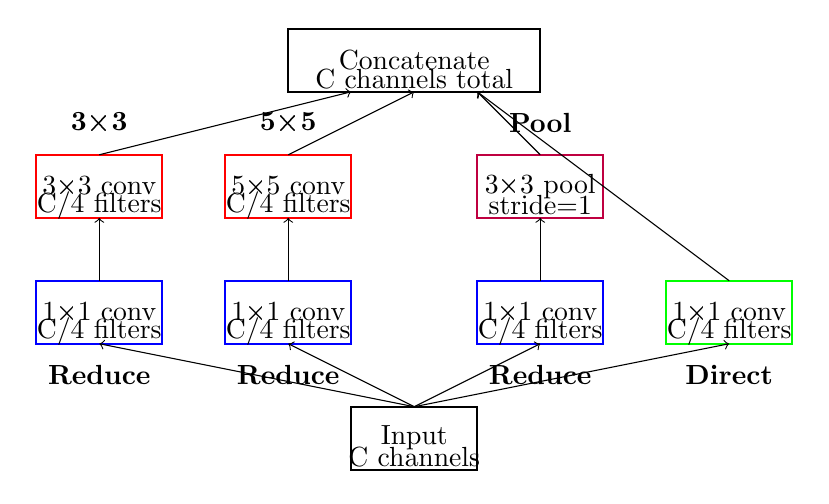
\begin{tikzpicture}[scale=0.8]
        % Input
        \draw[thick] (6,0) rectangle (8,1);
        \node at (7,0.5) {Input};
        \node at (7,0.2) {C channels};
        
        % 1x1 reduction branches
        \draw[blue, thick] (1,2) rectangle (3,3);
        \node at (2,2.5) {1×1 conv};
        \node at (2,2.2) {C/4 filters};
        
        \draw[blue, thick] (4,2) rectangle (6,3);
        \node at (5,2.5) {1×1 conv};
        \node at (5,2.2) {C/4 filters};
        
        \draw[blue, thick] (8,2) rectangle (10,3);
        \node at (9,2.5) {1×1 conv};
        \node at (9,2.2) {C/4 filters};
        
        % Direct 1x1 branch
        \draw[green, thick] (11,2) rectangle (13,3);
        \node at (12,2.5) {1×1 conv};
        \node at (12,2.2) {C/4 filters};
        
        % Main convolutions
        \draw[red, thick] (1,4) rectangle (3,5);
        \node at (2,4.5) {3×3 conv};
        \node at (2,4.2) {C/4 filters};
        
        \draw[red, thick] (4,4) rectangle (6,5);
        \node at (5,4.5) {5×5 conv};
        \node at (5,4.2) {C/4 filters};
        
        \draw[purple, thick] (8,4) rectangle (10,5);
        \node at (9,4.5) {3×3 pool};
        \node at (9,4.2) {stride=1};
        
        % Output concatenation
        \draw[thick] (5,6) rectangle (9,7);
        \node at (7,6.5) {Concatenate};
        \node at (7,6.2) {C channels total};
        
        % Arrows
        \draw[->] (7,1) -- (2,2);
        \draw[->] (7,1) -- (5,2);
        \draw[->] (7,1) -- (9,2);
        \draw[->] (7,1) -- (12,2);
        
        \draw[->] (2,3) -- (2,4);
        \draw[->] (5,3) -- (5,4);
        \draw[->] (9,3) -- (9,4);
        
        \draw[->] (2,5) -- (6,6);
        \draw[->] (5,5) -- (7,6);
        \draw[->] (9,5) -- (8,6);
        \draw[->] (12,3) -- (8,6);
        
        % Labels
        \node at (2,1.5) {\textbf{Reduce}};
        \node at (5,1.5) {\textbf{Reduce}};
        \node at (9,1.5) {\textbf{Reduce}};
        \node at (12,1.5) {\textbf{Direct}};
        
        \node at (2,5.5) {\textbf{3×3}};
        \node at (5,5.5) {\textbf{5×5}};
        \node at (9,5.5) {\textbf{Pool}};
    \end{tikzpicture}
    \end{center}
    
    \answer{The improved inception module uses 1×1 convolutions as "bottleneck" layers to reduce channel dimensions before expensive operations, controlling computational cost while maintaining multi-scale processing capability.}
    
    \explanation{
    \textbf{Scalability Problem in Naive Inception:}
    
    \textbf{Naive Approach:}
    Direct application of multiple kernel sizes to input with $C$ channels:
    \begin{itemize}
        \item $1 \times 1$ conv: produces $N_1$ channels
        \item $3 \times 3$ conv: produces $N_3$ channels  
        \item $5 \times 5$ conv: produces $N_5$ channels
        \item Pooling + conv: produces $N_p$ channels
        \item \textbf{Total output:} $N_1 + N_3 + N_5 + N_p$ channels
    \end{itemize}
    
    \textbf{Channel Explosion:}
    If we want meaningful representation:
    \begin{itemize}
        \item Each branch needs sufficient channels (e.g., 128+ channels each)
        \item Output becomes $4 \times 128 = 512$ channels
        \item Next layer input is 512 channels
        \item Grows exponentially through network depth
        \item Leads to parameter explosion and computational infeasibility
    \end{itemize}
    
    \textbf{Computational Cost Analysis:}
    
    For input $H \times W \times C$ and naive inception:
    \begin{itemize}
        \item $3 \times 3$ conv cost: $H \times W \times C \times N_3 \times 9$
        \item $5 \times 5$ conv cost: $H \times W \times C \times N_5 \times 25$ 
        \item Total cost grows as $O(C \times \text{total\_output\_channels})$
    \end{itemize}
    
    \textbf{1×1 Convolution Solution:}
    
    \textbf{Bottleneck Architecture:}
    \begin{enumerate}
        \item \textbf{Dimension Reduction:} Use $1 \times 1$ conv to reduce from $C$ to $C/4$ channels
        \item \textbf{Multi-scale Processing:} Apply $3 \times 3$, $5 \times 5$ on reduced dimensions
        \item \textbf{Dimension Restoration:} Each branch outputs $C/4$ channels
        \item \textbf{Concatenation:} $4 \times (C/4) = C$ total output channels
    \end{enumerate}
    
    \textbf{How 1×1 Convolution Works:}
    
    \textbf{Mathematical Operation:}
    For input $x \in \mathbb{R}^{H \times W \times C}$ and $1 \times 1$ filter $w \in \mathbb{R}^{1 \times 1 \times C \times C'}$:
    $$y_{i,j,k} = \sum_{c=1}^C w_{1,1,c,k} \cdot x_{i,j,c} + b_k$$
    
    \textbf{Effect:}
    \begin{itemize}
        \item Acts as learned linear combination across channels
        \item Reduces/increases channel dimension without affecting spatial dimensions
        \item Introduces non-linearity through ReLU activation
        \item Very efficient: only $C \times C'$ parameters per filter
    \end{itemize}
    
    \textbf{Computational Savings:}
    
    \textbf{Without Bottleneck (Naive):}
    \begin{itemize}
        \item $5 \times 5$ conv: $H \times W \times C \times (C/4) \times 25 = 6.25 \times HWC^2/4$
        \item Very expensive for large $C$
    \end{itemize}
    
    \textbf{With Bottleneck:}
    \begin{itemize}
        \item $1 \times 1$ reduction: $H \times W \times C \times (C/4) = HWC^2/4$
        \item $5 \times 5$ conv: $H \times W \times (C/4) \times (C/4) \times 25 = 25HWC^2/16$  
        \item Total: $HWC^2/4 + 25HWC^2/16 = HWC^2(4+25)/16 = 1.8 \times HWC^2$
        \item \textbf{Speedup:} $\frac{6.25}{1.8} \approx 3.5\times$ faster
    \end{itemize}
    
    \textbf{Key Benefits:}
    
    \textbf{1. Controlled Growth:}
    Output channels = Input channels, preventing exponential growth
    
    \textbf{2. Computational Efficiency:}
    Dramatic reduction in FLOPs while maintaining representational capacity
    
    \textbf{3. Feature Learning:}
    $1 \times 1$ convolutions learn optimal channel combinations
    
    \textbf{4. Scalability:}
    Can stack many inception modules without parameter explosion
    
    This bottleneck design became a fundamental principle in efficient CNN architectures, used in ResNet, MobileNet, and many others.
    }
    
    \item Explain GoogleNet's second contribution: "adding fully connected layers into the intermediate layers of the network." Discuss both benefits (gradient flow, multi-scale recognition) and drawbacks (reproducibility issues, loss of generalization) as mentioned by the professor. \hfill (10 marks)
    
    \answer{GoogleNet's auxiliary classifiers provide gradient flow improvements and multi-scale supervision but introduce training complexity and potential overfitting issues that limit their practical adoption.}
    
    \explanation{
    \textbf{Auxiliary Classifier Architecture:}
    
    \textbf{Placement:}
    \begin{itemize}
        \item Two auxiliary classifiers added at intermediate layers
        \item Located after inception modules 4a and 4d
        \item Each consists of: AvgPool → 1×1 Conv → FC → FC → Softmax
        \item Same 1000-class outputs as main classifier
    \end{itemize}
    
    \textbf{Training Procedure:}
    \begin{itemize}
        \item Total loss = Main loss + 0.3 × Aux1 loss + 0.3 × Aux2 loss
        \item All three classifiers trained simultaneously
        \item Auxiliary classifiers discarded during inference
        \item Only main classifier used for actual predictions
    \end{itemize}
    
    \textbf{Benefits:}
    
    \textbf{1. Improved Gradient Flow:}
    
    \textbf{Vanishing Gradient Problem:}
    \begin{itemize}
        \item GoogleNet has 22 layers - very deep for 2014
        \item Gradients become very small when backpropagated through many layers
        \item Early layers receive weak training signals
    \end{itemize}
    
    \textbf{Auxiliary Classifier Solution:}
    \begin{itemize}
        \item Provides direct gradient paths to intermediate layers
        \item Shorter backpropagation paths: gradients don't have to travel through all 22 layers
        \item Stronger training signals reach early and middle layers
        \item Helps combat vanishing gradients before ResNet's skip connections
    \end{itemize}
    
    \textbf{Mathematical Insight:}
    Gradient magnitude at layer $\ell$: $||\nabla_{\theta_\ell} \mathcal{L}|| \propto \prod_{i=\ell}^L ||\nabla a_i||$
    
    Auxiliary classifiers provide additional terms that don't require the full product.
    
    \textbf{2. Multi-Scale Feature Learning:}
    
    \textbf{Intermediate Supervision:}
    \begin{itemize}
        \item Forces intermediate layers to learn discriminative features
        \item Prevents early layers from becoming simple feature detectors
        \item Ensures useful representations at multiple network depths
        \item Creates multiple levels of abstraction for classification
    \end{itemize}
    
    \textbf{Feature Quality:}
    \begin{itemize}
        \item Middle layers must be good enough for classification
        \item Improves transferability of intermediate features
        \item Creates richer feature hierarchies
    \end{itemize}
    
    \textbf{3. Regularization Effect:}
    \begin{itemize}
        \item Acts as implicit regularization on intermediate features
        \item Prevents overfitting to specific feature combinations
        \item Encourages robust feature learning throughout network
    \end{itemize}
    
    \textbf{Drawbacks:}
    
    \textbf{1. Reproducibility Issues:}
    
    \textbf{Training Instability:}
    \begin{itemize}
        \item Three different loss terms with different dynamics
        \item Auxiliary loss weights (0.3) were manually tuned
        \item Sensitive to hyperparameter choices
        \item Different runs could converge to different solutions
    \end{itemize}
    
    \textbf{Implementation Complexity:}
    \begin{itemize}
        \item More complex training procedure
        \item Requires careful balancing of loss terms
        \item Harder to reproduce results across different frameworks
        \item Additional architectural components to implement
    \end{itemize}
    
    \textbf{2. Loss of Generalization:}
    
    \textbf{Overfitting Risk:}
    \begin{itemize}
        \item Auxiliary classifiers might overfit to training data
        \item Intermediate features become biased toward auxiliary tasks
        \item May hurt performance on transfer learning tasks
        \item Creates task-specific representations too early in network
    \end{itemize}
    
    \textbf{Feature Specialization:}
    \begin{itemize}
        \item Intermediate layers forced to be classifiers rather than feature extractors
        \item Reduces flexibility of learned representations
        \item May prevent learning of more general, transferable features
    \end{itemize}
    
    \textbf{3. Limited Practical Impact:}
    
    \textbf{Empirical Results:}
    \begin{itemize}
        \item Improvement was modest (1-2\% accuracy gain)
        \item Benefits didn't consistently transfer to other tasks
        \item ResNet's skip connections provided better gradient flow solution
        \item Most practitioners found auxiliary classifiers not worth the complexity
    \end{itemize}
    
    \textbf{Historical Impact:}
    
    \textbf{Lessons Learned:}
    \begin{itemize}
        \item Highlighted importance of gradient flow in deep networks
        \item Inspired better solutions (skip connections in ResNet)
        \item Showed that intermediate supervision can help but at a cost
        \item Demonstrated need for simpler, more principled approaches
    \end{itemize}
    
    \textbf{Modern Perspective:}
    Auxiliary classifiers are rarely used today because:
    \begin{itemize}
        \item ResNet skip connections solve gradient flow more elegantly
        \item Batch normalization helps with training stability
        \item Better optimizers (Adam, etc.) handle deep networks better
        \item Simpler architectures achieve better results
    \end{itemize}
    
    GoogleNet's auxiliary classifiers were innovative but ultimately a stepping stone to better solutions for training very deep networks.
    }
\end{enumerate}

\newpage
\paragraph{Question 6. ResNet and Skip Connections}{\hfill (25 marks)}\\
The professor explained the key insight: "After a certain number of layers performance doesn't improve... it actually becomes even worse" and ResNet's solution using skip connections.

\begin{enumerate}[(a)]
    \item Analyze the professor's explanation of why deeper networks perform worse: "when you multiply all those gradients through all of these layers you don't get useful gradients to the earlier parts of the network." Explain why this isn't simply overfitting. \hfill (8 marks)
    
    \answer{The degradation problem in deep networks is fundamentally different from overfitting - it's a training optimization problem where even training accuracy degrades, caused by vanishing gradients and optimization difficulties rather than generalization failure.}
    
    \explanation{
    \textbf{Empirical Observation - The Degradation Problem:}
    
    \textbf{Experimental Evidence:}
    \begin{itemize}
        \item 20-layer network: 91.25\% training accuracy, 89.43\% test accuracy
        \item 56-layer network: 90.16\% training accuracy, 87.23\% test accuracy
        \item Deeper network performs worse on \textbf{both} training and test sets
        \item This contradicts typical overfitting patterns
    \end{itemize}
    
    \textbf{Why It's Not Overfitting:}
    
    \textbf{Overfitting Characteristics:}
    \begin{itemize}
        \item Training accuracy increases while test accuracy decreases
        \item Model memorizes training data but fails to generalize
        \item More parameters → better training fit, worse test performance
        \item Training loss continues to decrease
    \end{itemize}
    
    \textbf{Degradation Problem Characteristics:}
    \begin{itemize}
        \item \textbf{Both} training and test accuracy degrade
        \item Training loss stops decreasing or even increases
        \item More parameters → worse performance on all metrics
        \item Clear optimization failure, not generalization failure
    \end{itemize}
    
    \textbf{Vanishing Gradient Analysis:}
    
    \textbf{Mathematical Foundation:}
    For a deep network with $L$ layers, the gradient at layer $\ell$ is:
    $$\frac{\partial \mathcal{L}}{\partial \theta_\ell} = \frac{\partial \mathcal{L}}{\partial a_L} \prod_{i=\ell+1}^L \frac{\partial a_i}{\partial a_{i-1}} \frac{\partial a_\ell}{\partial \theta_\ell}$$
    
    \textbf{Chain Rule Problem:}
    The gradient involves a product of $L-\ell$ terms. Each term $\frac{\partial a_i}{\partial a_{i-1}}$ can be:
    \begin{itemize}
        \item Small ($< 1$): Product approaches zero exponentially
        \item Large ($> 1$): Product explodes exponentially
        \item Both cases make training unstable
    \end{itemize}
    
    \textbf{Activation Function Impact:}
    
    \textbf{Sigmoid/Tanh:}
    \begin{itemize}
        \item Derivative range: $(0, 0.25]$ for sigmoid
        \item Product of many small terms → vanishing gradients
        \item Early layers receive virtually no training signal
    \end{itemize}
    
    \textbf{ReLU:}
    \begin{itemize}
        \item Derivative: 1 (if $x > 0$) or 0 (if $x \leq 0$)
        \item Helps with vanishing gradients but creates "dying ReLU" problem
        \item Still suffers from optimization difficulties in very deep networks
    \end{itemize}
    
    \textbf{Optimization Landscape Perspective:}
    
    \textbf{Loss Surface Complexity:}
    \begin{itemize}
        \item Deeper networks have more complex loss landscapes
        \item More local minima and saddle points
        \item Harder for optimizers to find good solutions
        \item Path dependence in optimization trajectory
    \end{itemize}
    
    \textbf{Identity Mapping Problem:}
    Deep networks should theoretically perform at least as well as shallow ones:
    \begin{itemize}
        \item Extra layers could learn identity mappings
        \item In practice, learning identity mappings is difficult
        \item Networks struggle to approximate $H(x) = x$ when needed
        \item This suggests optimization rather than representational limitations
    \end{itemize}
    
    \textbf{Empirical Evidence Against Overfitting:}
    
    \textbf{1. Training Performance Degradation:}
    If it were overfitting, training accuracy should still be high or increasing.
    
    \textbf{2. Consistent Across Datasets:}
    The problem appears on various datasets, not just specific overfitting scenarios.
    
    \textbf{3. Architecture Independence:}
    Different architectures show similar degradation patterns.
    
    \textbf{4. Regularization Doesn't Help:}
    Standard overfitting solutions (dropout, weight decay) don't solve the degradation problem.
    
    This analysis led to the insight that the fundamental problem is optimization difficulty, not overfitting, which motivated the skip connection solution in ResNet.
    }
    
    \item Draw a ResNet block and explain the professor's description: "in forward pass we have a function of the input as well as the identity being propagated" and "in backward pass gradient will flow through two paths." \hfill (10 marks)

    \begin{center}
    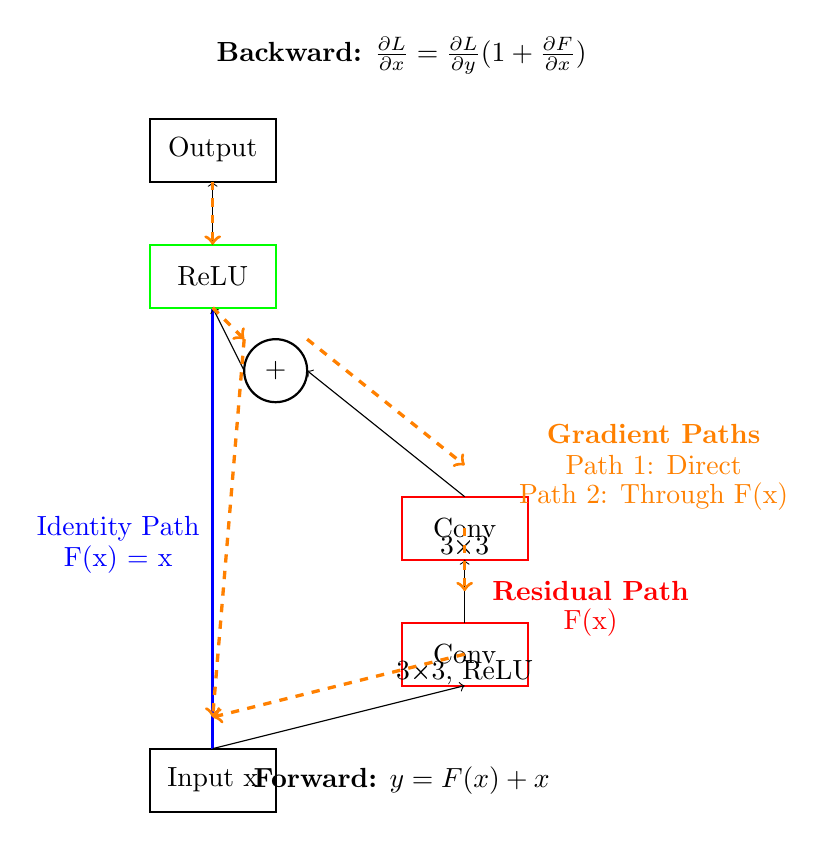
\begin{tikzpicture}[scale=0.8]
        % Input
        \draw[thick] (2,0) rectangle (4,1);
        \node at (3,0.5) {Input x};
        
        % Identity path (skip connection)
        \draw[blue, very thick] (3,1) -- (3,8);
        \node[blue] at (1.5,4.5) {Identity Path};
        \node[blue] at (1.5,4) {F(x) = x};
        
        % Function path - first conv
        \draw[red, thick] (6,2) rectangle (8,3);
        \node at (7,2.5) {Conv};
        \node at (7,2.2) {3×3, ReLU};
        
        % Function path - second conv  
        \draw[red, thick] (6,4) rectangle (8,5);
        \node at (7,4.5) {Conv};
        \node at (7,4.2) {3×3};
        
        % Addition
        \draw[thick] (4,7) circle (0.5);
        \node at (4,7) {+};
        
        % Final ReLU
        \draw[green, thick] (2,8) rectangle (4,9);
        \node at (3,8.5) {ReLU};
        
        % Output
        \draw[thick] (2,10) rectangle (4,11);
        \node at (3,10.5) {Output};
        
        % Forward pass arrows
        \draw[->] (3,1) -- (7,2);
        \draw[->] (7,3) -- (7,4);
        \draw[->] (7,5) -- (4.5,7);
        \draw[->] (3.5,7) -- (3,8);
        \draw[->] (3,9) -- (3,10);
        
        % Gradient flow arrows (dashed, different color)
        \draw[orange, dashed, very thick, ->] (3,10) -- (3,9);
        \draw[orange, dashed, very thick, ->] (3,8) -- (3.5,7.5);
        \draw[orange, dashed, very thick, ->] (4.5,7.5) -- (7,5.5);
        \draw[orange, dashed, very thick, ->] (7,4.5) -- (7,3.5);
        \draw[orange, dashed, very thick, ->] (7,2.5) -- (3,1.5);
        
        % Direct gradient path
        \draw[orange, dashed, very thick, ->] (3.5,7.5) -- (3,1.5);
        
        % Labels
        \node[red] at (9,3.5) {\textbf{Residual Path}};
        \node[red] at (9,3) {F(x)};
        
        \node[orange] at (10,6) {\textbf{Gradient Paths}};
        \node[orange] at (10,5.5) {Path 1: Direct};
        \node[orange] at (10,5) {Path 2: Through F(x)};
        
        % Mathematical formulation
        \node at (6,0.5) {\textbf{Forward:} $y = F(x) + x$};
        \node at (6,12) {\textbf{Backward:} $\frac{\partial L}{\partial x} = \frac{\partial L}{\partial y}(1 + \frac{\partial F}{\partial x})$};
    \end{tikzpicture}
    \end{center}
    
    \answer{ResNet blocks combine a residual function F(x) with an identity skip connection, enabling gradient flow through both transformed and direct paths during backpropagation.}
    
    \explanation{
    \textbf{ResNet Block Architecture:}
    
    \textbf{Forward Pass Components:}
    \begin{enumerate}
        \item \textbf{Input:} $x$ (from previous layer)
        \item \textbf{Residual Function:} $F(x)$ (typically 2-3 conv layers)
        \item \textbf{Skip Connection:} Direct path carrying $x$
        \item \textbf{Addition:} Element-wise sum $F(x) + x$
        \item \textbf{Output:} $y = F(x) + x$ (usually followed by ReLU)
    \end{enumerate}
    
    \textbf{Forward Pass Mathematics:}
    
    \textbf{Traditional Deep Network:}
    $$y = H(x)$$
    Network must learn the full mapping $H(x)$ from scratch.
    
    \textbf{ResNet Formulation:}
    $$y = F(x) + x$$
    where:
    \begin{itemize}
        \item $F(x)$ is the residual function (learned by conv layers)
        \item $x$ is the identity mapping (skip connection)
        \item Network only needs to learn the residual $F(x) = H(x) - x$
    \end{itemize}
    
    \textbf{Key Insight:} Learning $F(x) = H(x) - x$ is easier than learning $H(x)$ directly, especially when $H(x) \approx x$ (near-identity mappings).
    
    \textbf{Backward Pass - Dual Gradient Paths:}
    
    \textbf{Gradient Computation:}
    Using chain rule on $y = F(x) + x$:
    $$\frac{\partial \mathcal{L}}{\partial x} = \frac{\partial \mathcal{L}}{\partial y} \frac{\partial y}{\partial x} = \frac{\partial \mathcal{L}}{\partial y} \left(\frac{\partial F(x)}{\partial x} + \frac{\partial x}{\partial x}\right) = \frac{\partial \mathcal{L}}{\partial y} \left(\frac{\partial F(x)}{\partial x} + 1\right)$$
    
    \textbf{Two Gradient Paths:}
    
    \textbf{Path 1 - Direct (Identity):}
    \begin{itemize}
        \item Contribution: $\frac{\partial \mathcal{L}}{\partial y} \cdot 1$
        \item Always present regardless of $F(x)$
        \item Provides unimpeded gradient flow
        \item Prevents vanishing gradients
    \end{itemize}
    
    \textbf{Path 2 - Residual:}
    \begin{itemize}
        \item Contribution: $\frac{\partial \mathcal{L}}{\partial y} \cdot \frac{\partial F(x)}{\partial x}$
        \item Depends on learned residual function
        \item Can vanish if $F(x)$ saturates
        \item Provides additional learning signal
    \end{itemize}
    
    \textbf{Benefits of Dual Path Design:}
    
    \textbf{1. Gradient Flow Guarantee:}
    Even if $\frac{\partial F(x)}{\partial x} \rightarrow 0$, gradients still flow through identity path:
    $$\frac{\partial \mathcal{L}}{\partial x} = \frac{\partial \mathcal{L}}{\partial y}(0 + 1) = \frac{\partial \mathcal{L}}{\partial y}$$
    
    \textbf{2. Optimization Advantage:}
    \begin{itemize}
        \item If optimal mapping is identity: $F(x) \rightarrow 0$ (easier than learning $H(x) = x$)
        \item If optimal mapping is complex: $F(x)$ learns the residual
        \item Network can adaptively choose between identity and transformation
    \end{itemize}
    
    \textbf{3. Multi-Scale Learning:}
    \begin{itemize}
        \item Identity path preserves low-level features
        \item Residual path learns new transformations
        \item Combination enables both preservation and transformation
    \end{itemize}
    
    \textbf{Training Dynamics:}
    
    \textbf{Early Training:}
    \begin{itemize}
        \item $F(x)$ starts near zero (due to initialization)
        \item Output $y \approx x$ (near-identity)
        \item Strong gradient flow enables early layer training
    \end{itemize}
    
    \textbf{During Training:}
    \begin{itemize}
        \item $F(x)$ gradually learns useful residuals
        \item Identity path maintains stable gradient flow
        \item Network learns both to preserve and transform features
    \end{itemize}
    
    \textbf{Theoretical Foundation:}
    
    \textbf{Highway Networks Connection:}
    ResNet can be viewed as a special case of highway networks with:
    \begin{itemize}
        \item Transform gate: $T = 1$ (always transform)
        \item Carry gate: $C = 1$ (always carry)
        \item Fixed gating removes learning overhead
    \end{itemize}
    
    This dual-path design revolutionized deep learning by solving the degradation problem and enabling training of networks with hundreds of layers.
    }
    
    \item The professor mentioned two interpretations of why ResNet works: the "smoother loss function" hypothesis and viewing ResNet as "an ensemble of multiple sub networks." Explain both interpretations and discuss why "there is no theorem showing this." \hfill (7 marks)
    
    \answer{ResNet's success has multiple theoretical explanations including loss landscape smoothing and ensemble-like behavior, but the lack of formal proofs reflects the general challenge of theoretically understanding deep neural networks.}
    
    \explanation{
    \textbf{Interpretation 1: Smoother Loss Function Hypothesis}
    
    \textbf{Core Idea:}
    Skip connections fundamentally change the loss landscape, making it smoother and easier to optimize.
    
    \textbf{Mathematical Intuition:}
    
    \textbf{Traditional Network Loss Surface:}
    \begin{itemize}
        \item Highly non-convex with many local minima
        \item Sharp valleys and plateaus
        \item Gradient descent can get trapped in poor local optima
        \item Small parameter changes can cause large loss changes
    \end{itemize}
    
    \textbf{ResNet Loss Surface:}
    \begin{itemize}
        \item Skip connections provide "shortcuts" across the loss landscape
        \item Smoother gradients due to identity path contribution
        \item Fewer sharp local minima
        \item More predictable optimization behavior
    \end{itemize}
    
    \textbf{Empirical Evidence:}
    \begin{itemize}
        \item Loss visualization studies show smoother landscapes for ResNets
        \item More consistent convergence across different initializations
        \item Less sensitivity to learning rate choices
        \item Better optimization even with simple SGD
    \end{itemize}
    
    \textbf{Gradient Smoothing Effect:}
    The dual gradient paths create more stable gradient flow:
    $$\frac{\partial \mathcal{L}}{\partial x} = \frac{\partial \mathcal{L}}{\partial y}\left(1 + \frac{\partial F(x)}{\partial x}\right)$$
    
    The "+1" term ensures gradients never completely vanish, providing consistent optimization signals.
    
    \textbf{Interpretation 2: Ensemble of Sub-Networks}
    
    \textbf{Core Idea:}
    ResNet can be viewed as an exponential ensemble of sub-networks of different depths, each taking different paths through the skip connections.
    
    \textbf{Mathematical Framework:}
    
    For a ResNet with $n$ blocks, each with a skip connection, there are $2^n$ possible paths:
    \begin{itemize}
        \item Each block can either apply transformation $F_i(x)$ or skip it
        \item Path through blocks 1,3,5: $x \rightarrow F_1(x) \rightarrow F_3(F_1(x)) \rightarrow F_5(F_3(F_1(x)))$
        \item Total computation is sum over all paths weighted by their contributions
    \end{itemize}
    
    \textbf{Unraveled View:}
    A ResNet can be written as:
    $$y = \sum_{\text{paths } p} \prod_{i \in p} F_i(x)$$
    
    where the sum is over all possible paths through the network.
    
    \textbf{Ensemble Properties:}
    
    \textbf{1. Implicit Averaging:}
    \begin{itemize}
        \item Different paths contribute different "votes" to final prediction
        \item Naturally provides ensemble-like robustness
        \item Multiple depths provide multiple levels of abstraction
    \end{itemize}
    
    \textbf{2. Graceful Degradation:}
    \begin{itemize}
        \item If some blocks fail or perform poorly, other paths compensate
        \item Network is robust to individual component failures
        \item Training naturally balances path contributions
    \end{itemize}
    
    \textbf{3. Multi-Scale Processing:}
    \begin{itemize}
        \item Short paths provide coarse features
        \item Long paths provide detailed transformations  
        \item Ensemble captures features at multiple scales
    \end{itemize}
    
    \textbf{Empirical Support:}
    
    \textbf{Path Analysis Studies:}
    \begin{itemize}
        \item Gradient flow primarily through shorter paths during training
        \item Longer paths contribute less but still matter for performance
        \item Removing random subsets of blocks degrades performance gracefully
        \item Path importance follows specific distribution patterns
    \end{itemize}
    
    \textbf{Why "There is No Theorem Showing This":}
    
    \textbf{1. Complexity of Deep Networks:}
    
    \textbf{Mathematical Challenges:}
    \begin{itemize}
        \item Deep networks are highly non-linear systems
        \item Interactions between layers are complex and input-dependent
        \item Optimization dynamics involve stochastic processes (SGD, mini-batches)
        \item High-dimensional parameter spaces resist theoretical analysis
    \end{itemize}
    
    \textbf{2. Multiple Concurrent Effects:}
    \begin{itemize}
        \item Skip connections affect optimization, generalization, and representation simultaneously
        \item Hard to isolate individual causal mechanisms
        \item Different explanations may all be partially correct
        \item Interactions between effects complicate theoretical analysis
    \end{itemize}
    
    \textbf{3. Empirical vs. Theoretical Understanding:}
    
    \textbf{Deep Learning Theory Gap:}
    \begin{itemize}
        \item Most successful deep learning innovations discovered empirically
        \item Theory often lags behind practical breakthroughs
        \item Theoretical tools are still developing for deep networks
        \item Phenomena may be too complex for current mathematical frameworks
    \end{itemize}
    
    \textbf{4. Statistical vs. Deterministic Analysis:}
    \begin{itemize}
        \item Deep learning involves high-dimensional statistics
        \item Traditional optimization theory assumes deterministic settings
        \item Real networks trained with noisy, finite data
        \item Generalization requires understanding of statistical learning theory
    \end{itemize}
    
    \textbf{Current State:}
    
    \textbf{Partial Results:}
    \begin{itemize}
        \item Some theoretical insights for specific cases (linear networks, infinite width)
        \item Empirical studies support various hypotheses
        \item No unified theory explaining all aspects of ResNet success
        \item Active area of ongoing research
    \end{itemize}
    
    \textbf{Practical Implications:}
    \begin{itemize}
        \item Architecture design remains largely empirical
        \item Multiple theoretical perspectives provide useful intuitions
        \item Importance of ablation studies and empirical validation
        \item Need for continued theoretical research in deep learning
    \end{itemize}
    
    The lack of formal theorems reflects the broader challenge in deep learning theory - understanding why these networks work so well remains an active and important research area.
    }
\end{enumerate}

\vfill
\begin{center}{\bf END OF PAPER}\end{center>
\end{document}